\subsection{Capacidade dada matriz}
% bilmes Homework 5 - q7

\begin{questions}
\question{
Mostre que a capacidade do canal com probabilidade de transmissão dada pela matriz 
\begin{equation}
        P_{y \vert x} = \begin{bmatrix} 2/3 & 1/3 & 0 \\ 1/3 & 1/3 & 1/3 \\ 0 & 1/3 & 2/3 \end{bmatrix}
\end{equation}
é alcançada por uma distribuição que coloca probabilidade zero em um dos símbolos de entrada. Qual é a capacidade deste canal? Por qual razão esta letra não é utilizada?

}

\begin{solution}

Seja $X \sim p = (p_1, p_2, p_3)$. As probabilidades dos 3 símbolos de saída
serão dadas por $q = (q_1, q_2, q_3)$, onde $q_1 = \frac{2}{3} p_1 + \frac{1}{3} p_2$,
$q_2 = \frac{1}{3}$ e $q_3 = \frac{1}{3} p_2 + \frac{2}{3} p_3$. Desta forma, teremos

\begin{eqnarray}
I(X;Y) &=& \underbrace{H(Y)}_{H\left( \frac{2}{3} p_1 + \frac{1}{3} p_2, \frac{1}{3}, \frac{1}{3} p_2 + \frac{2}{3} p_3 \right)} - \underbrace{H(Y|X)}_{\sum_x p(x) H(Y|X = x)} \nonumber \\
        &=& H\left( \frac{2}{3} p_1 + \frac{1}{3} p_2, \frac{1}{3}, \frac{1}{3} p_2 + \frac{2}{3} p_3 \right) - p_1 H\left( \frac{2}{3}, \frac{1}{3} \right) - p_2 \log 3 - p_3 H\left( \frac{2}{3}, \frac{1}{3} \right) \nonumber \\
        && \text{utilizando que } p_2 = 1 - p_1 - p_3 \nonumber \\
        &=& H\left( \frac{1}{3} + \frac{1}{3} (p_1 - p_3), \frac{1}{3}, \frac{1}{3} - \frac{1}{3} (p_1 - p_3) \right) -
        (p_1 + p_3) H\left( \frac{2}{3}, \frac{1}{3} \right) - (1-p_1-p_3) \log 3 
\end{eqnarray}

Se fixarmos $p_1 + p_3$, o segundo e terceiro termo da equação acima ficarão fixos, assim 
a informação mútua será maximizada quando o primeiro termo for maximizado, ou seja,
quando $p_1 = p_3$. Neste caso, teremos
\begin{eqnarray}
I(X;Y) &=&  \underbrace{H\left( \frac{1}{3},  \frac{1}{3},  \frac{1}{3} \right)}_{= \log 3 } - (p_1 + p_3) \underbrace{ H\left( \frac{2}{3}, \frac{1}{3} \right) }_{= \log 3 - \frac{2}{3} } - (1- p_1 - p_3) \log 3 \nonumber \\
        &=&  \log 3 - (p_1 + p_3) \left( \log 3 - \frac{2}{3} \right)  - (1- p_1 - p_3) \log 3 \nonumber  \\
        &=& (p_1 + p_3) \left( \log 3 -   \log 3 + \frac{2}{3} \right) = (p_1 + p_3) \frac{2}{3} 
\end{eqnarray}


A informação mútua será máxima quando maximizarmos $p_1 + p_3$, sujeito a $p_1 = p_3$, ou seja,
quando $p_1 = p_3 = \frac{1}{2}$ e por conseguinte $p_2 = 0$. Teremos assim $C = \frac{2}{3}$,
que será atingida com a distribuição $p = (\frac{1}{2}, 0, \frac{1}{2})$.

\begin{lstlisting}[language=Octave]
function H=entropy(p)
H = (-sum(p.*log2(p)));
endfunction

p1=linspace(0,1,21);
p3=linspace(0,1,21);
I=[]; 
for i=1:length(p1), for j=1:length(p3), 
  if(p1(i)+p3(j)<=1), 
    I(i,j) = entropy( [1/3+1/3*(p1(i)-p3(j)), 1/3, 1/3 - 1/3*(p1(i)-p3(j)) ] ) - ...
        (p1(i)+p3(j))*entropy([2/3,1/3]) - (1 - p1(i) - p3(j)) * log2(3); 
  endif; 
endfor; endfor;

[i,j] = find(I==(max(max(I))));
figure; mesh(p1,p3,I,'facecolor', 'none', 'edgecolor', 'b');
xlabel('p1'); ylabel('p3'); zlabel('I(X;Y)');
hold on; plot3(p1(i),p3(j),I(i,j),'ok','markerfacecolor','k','markersize',8);
text(p1(i)+0.02,p3(j)+0.02,I(i,j)+0.02, ... 
   cstrcat('(',num2str(p1(i)),',',num2str(p3(j)),',',num2str(I(i,j),'%.2f'),')'));
print figure1.pdf
\end{lstlisting}

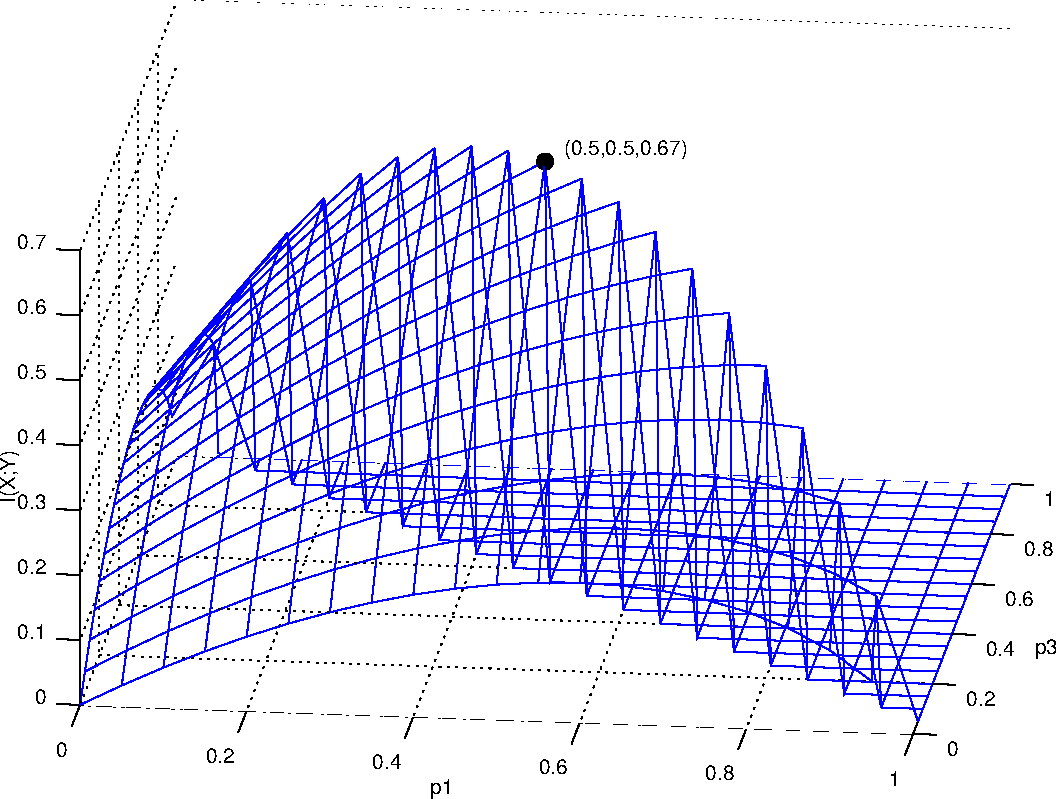
\includegraphics[width=0.5\textwidth]{../images/figure1.pdf}



\end{solution}
\end{questions}

